\subsection{Basis idee}
Het spel heeft twee teams die ieder een hoofdgebouw hebben. Elk team bestaat uit een of meerdere spelers. Doel van het spel is om het hoofdgebouw van de tegenstander te vernietigen. De spelers behoren tot een van beide teams en hebben laser geweren om de tegenstanders dood te schieten en torens aan te vallen. Torens kunnen door spelers worden neergezet op de map. Deze torens kosten gold om te bouwen. De spelers verdienen gold in een gezamenlijke kas door mining installations te bouwen over mining spots en door tegenstanders en hun torens dood/kapot te schieten. Als een speler dood gaat of een toren kapot gaat, zal deze een muntje droppen dat vervolgens door alle spelers kan worden opgepakt.

\subsection{Terrein}
Het terrein kan in wezen allerlei vormen hebben, voorwaarde is dat het een eerlijk terrein is voor beide teams, een team mag dus geen voordeel hebben dankzij de kaart. Een goede manier waarop dit te verhinderen is, is door het terrein symmetrisch te maken. Op het terrein zijn twee hoofdgebouwen geplaatst, voor beide teams een hoofdgebouw. Beide hoofdgebouwen worden al dan niet beschermd door initi\"ele torens. Over het terrein zijn een aantal mining spots verdeeld. Deze zijn eerlijk verdeeld over de kaart. Andere obstakels mogen aanwezig zijn, maar zijn niet noodzakelijkerwijs aanwezig.

\begin{figure}
\center
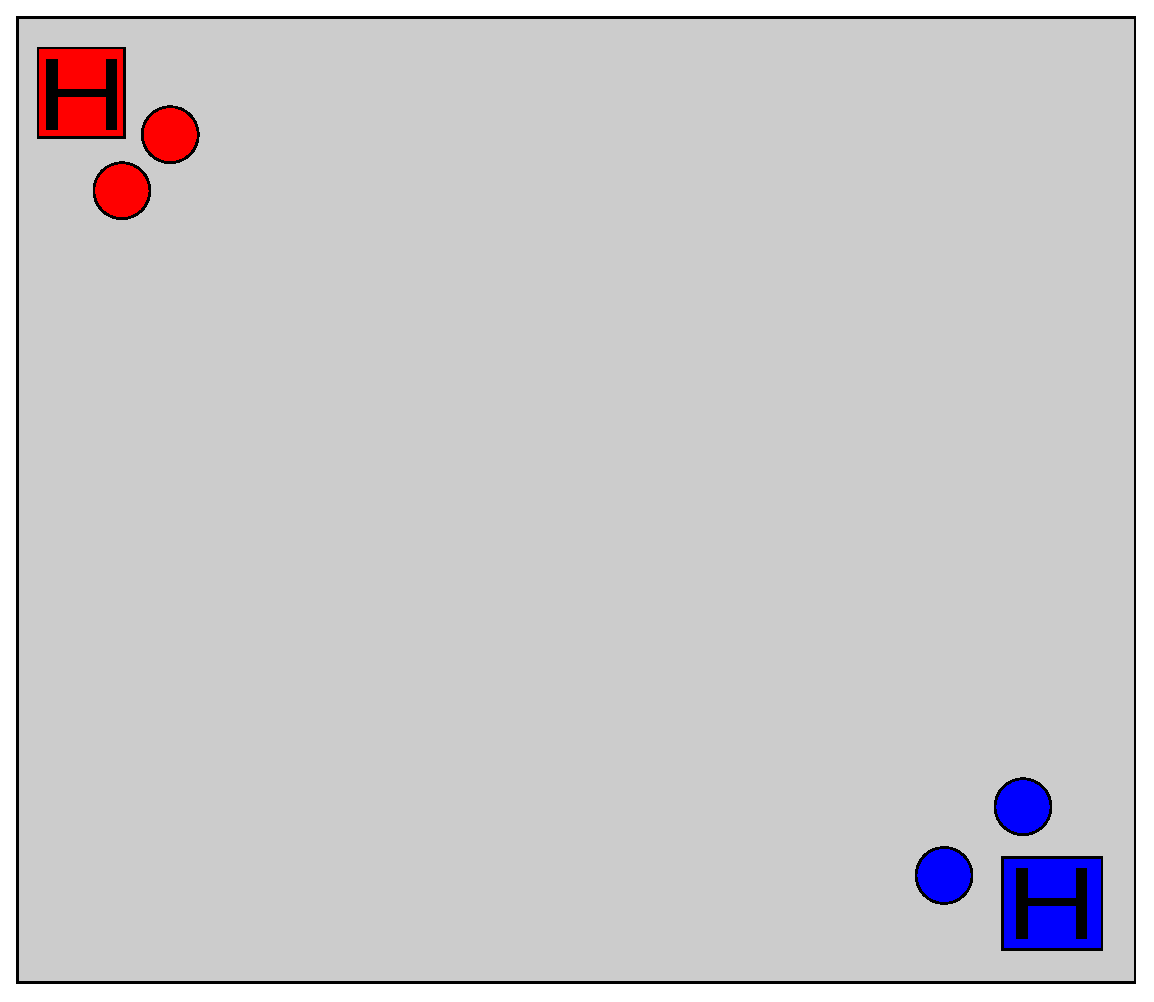
\includegraphics[width = 10cm]{Map1.eps}
\caption{Mogelijke kaart}
\label{fig:hist}
\end{figure}

\begin{figure}
\center
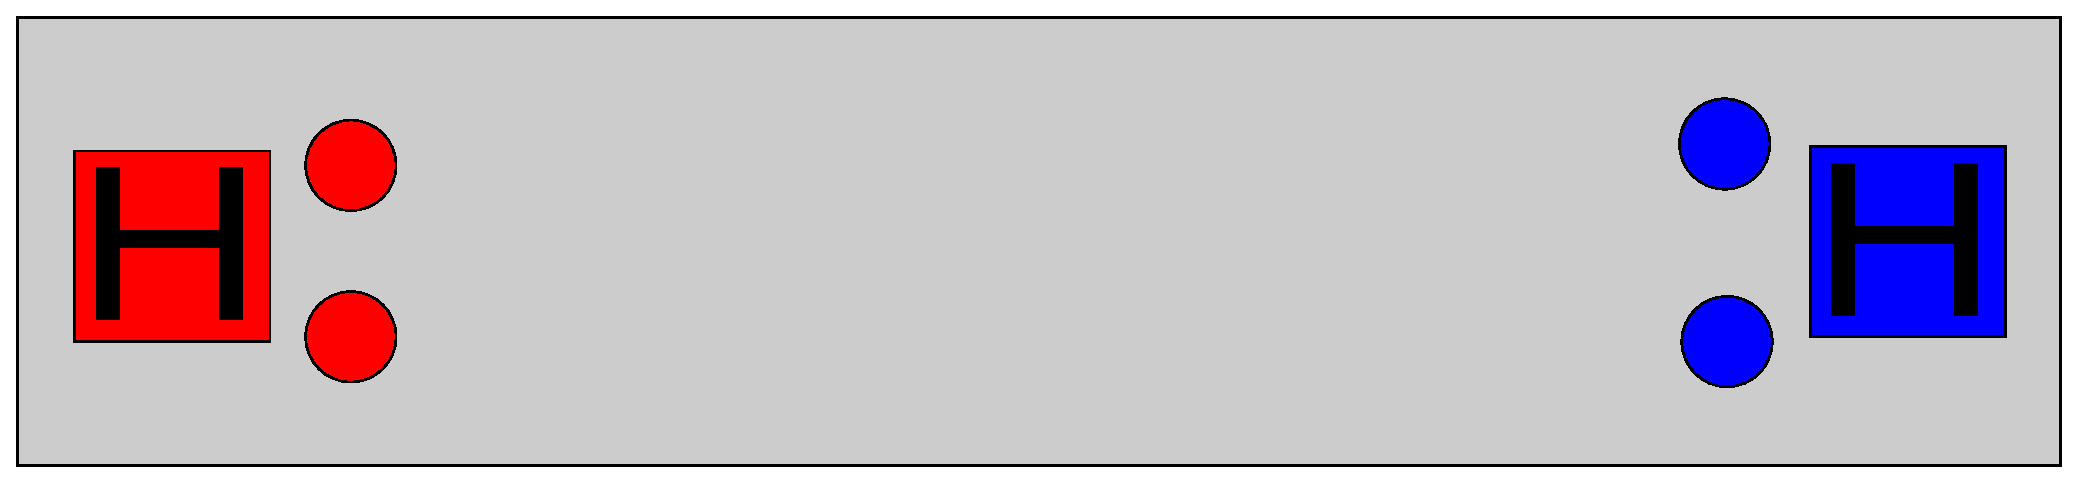
\includegraphics[width = 10cm]{Map2.eps}
\caption{Mogelijke kaart}
\label{fig:hist}
\end{figure}

\subsection{Spelers}
Een speler behoort tot een van beide teams, dit wordt duidelijk gemaakt door het kleuren schema van de speler. De speler heeft een laser geweer waarmee hij op andere spelers en torens kan schieten om deze te vernietigen. Als een speler dood gaat zal hij na een bepaalde tijd respawnen. Ook kan een speler gebouwen bouwen, hiervoor gebruikt hij gold uit de kas van het team. De spelers kunnen in het 2d vlak bewegen. De spelers besturen hun character in een 3rd person view.

\subsection{Gebouwen}
Er zijn drie soorten gebouwen: Torens (gebouwen die op spelers en andere gebouwen in hun bereik kunnen schieten), Mining installations (gebouwen die over een mining spot kunnen worden gebouwd om de inkomsten van jouw team te vergroten) en een Hoofdgebouw (het belangrijkste gebouw voor het team, als dit gebouw kapot is, heeft het bijbehorende team verloren). Alle gebouwen behoren tot een van beide teams, dit wordt duidelijk gemaakt door middel van het kleuren schema van het gebouw.

\subsection{Droppables}
Er is maar een soort droppable: een muntje. Een muntje wordt gedropt door spelers die dood gaan en torens die kapot gaan. Een muntje heeft een bepaalde waarde in gold. Een muntje kan opgepakt worden door alle spelers, de waarde van het muntje zal dan toegevoegd worden aan de kas van het team.

\subsection{Optioneel}
We hebben ook een aantal plannen voor uitbreiding van het spel, vooral om het uitgebreider te maken en leuker om te spelen. De volgende idee\"en staan op ons lijstje:
\begin{itemize}
  \item Minimap, zodat spelers een globaal overzicht krijgen van wat er in de arena gebeurt.
  \item Walls, als gebouw. Een wall als gebouw met lage kosten geeft wat meer opties voor een team om hun hoofdgebouw/mining spot te beschermen of een veilige plek te hebben om de tegenstander aan te vallen.
  \item Builder minions, computergestuurde robotjes die vanuit de basis komen om een gebouw te bouwen als de speler daar opdracht toe geeft. Hierdoor
duurt het langer om een gebouw te bouwen als de afstand vanaf je hoofdgebouw groter is en als de builder minions dood worden geschoten wordt het bouwen vertraagd.
  \item Attack minions, computergestuurde robotjes die kunnen worden gekocht en vanuit het hoofdgebouw een aanval doen op gebouwen van de tegenstander en alles wat ze tegen komen.
  \item Upgrades, de spelers ontwikkelen tijdens het spel en verdienen punten door het doodschieten van spelers/minions en het kapotschieten van gebouwen. Hiermee kunnen de spelers bijvoorbeeld hun stats upgraden of nieuwe wapens of uitrusting kopen bij het hoofdgebouw.
\end{itemize}